\documentclass[border={-4pt -6pt -4pt -9pt}]{standalone}

\usepackage{hyperref}
\usepackage{tikz}

\usetikzlibrary{decorations.pathreplacing,
  arrows,
  calc,
  decorations.pathmorphing,
  decorations.pathreplacing,
  decorations.markings,
  positioning,
  shapes,
  3d
}

\ifpdf
% Ensure reproducible output
\pdfinfoomitdate=1
\pdfsuppressptexinfo=-1
\pdftrailerid{}
\hypersetup{
  pdfcreator={},
  pdfproducer={}
}
\fi

\begin{document}
\begin{tikzpicture}
  \node at (3.175, 4.75) {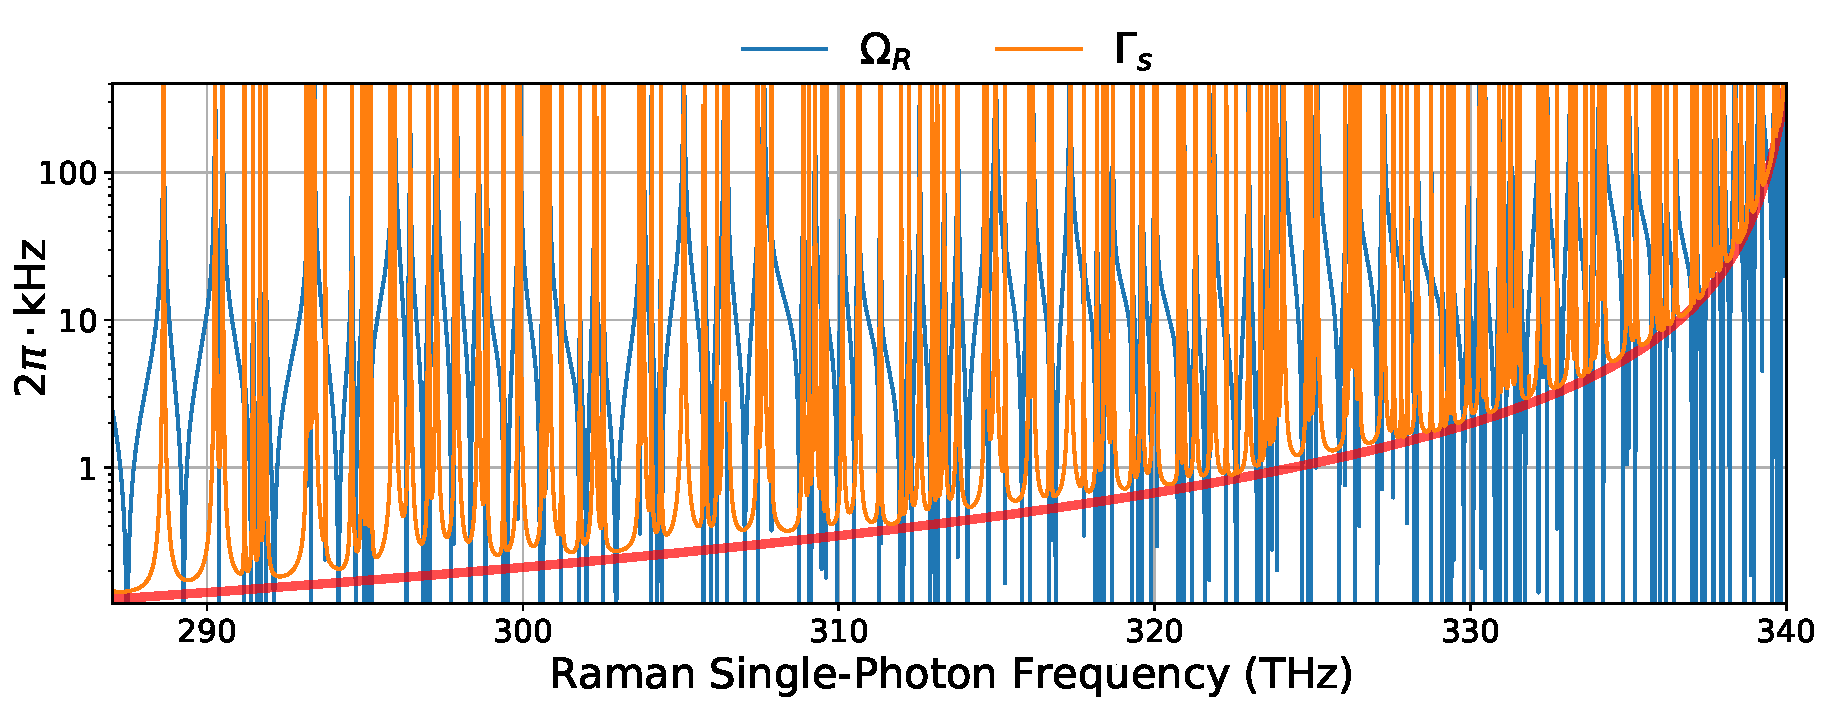
\includegraphics[width=12.8cm]{raman_transfer_theory_ratio_full.pdf}};
  \node at (-2.8, 6.65) {\scriptsize (\textbf{A})};
  \node at (0.0, 0) {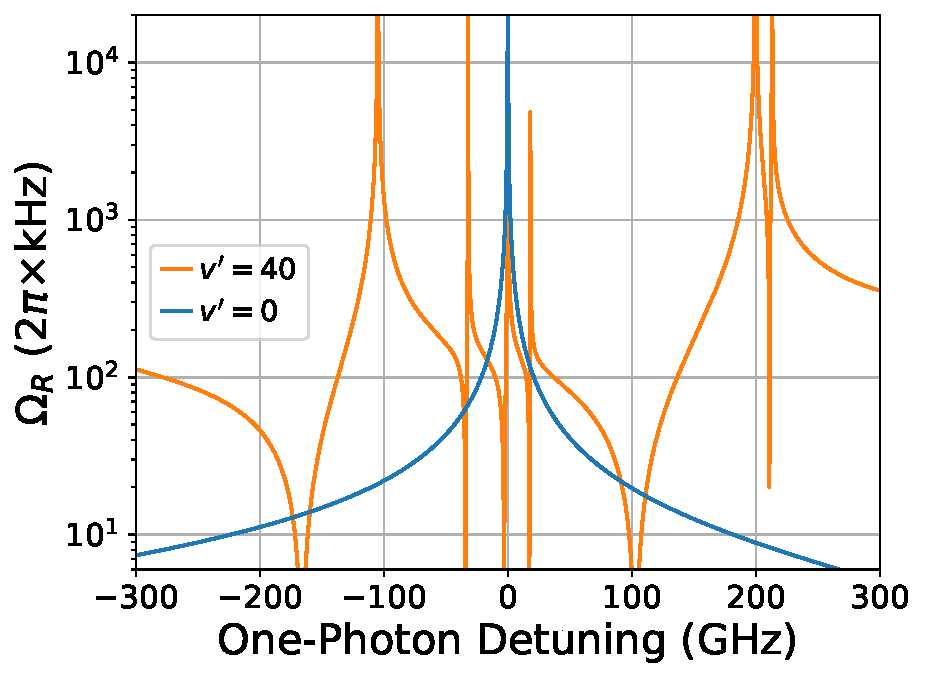
\includegraphics[width=6.4cm]{raman_transfer_theory_ratio_omega.pdf}};
  \node at (-1.95, 2.0) {\scriptsize (\textbf{B})};
  \node at (6.35, 0) {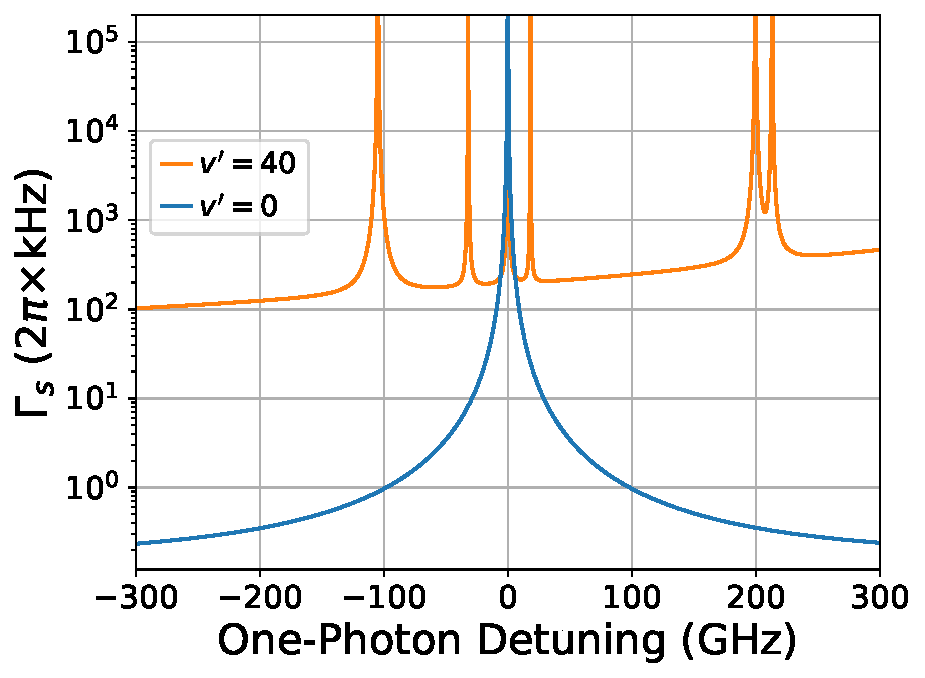
\includegraphics[width=6.4cm]{raman_transfer_theory_ratio_gamma.pdf}};
  \node at (4.4, 2.0) {\scriptsize (\textbf{C})};
  \node at (3.175, -4.65) {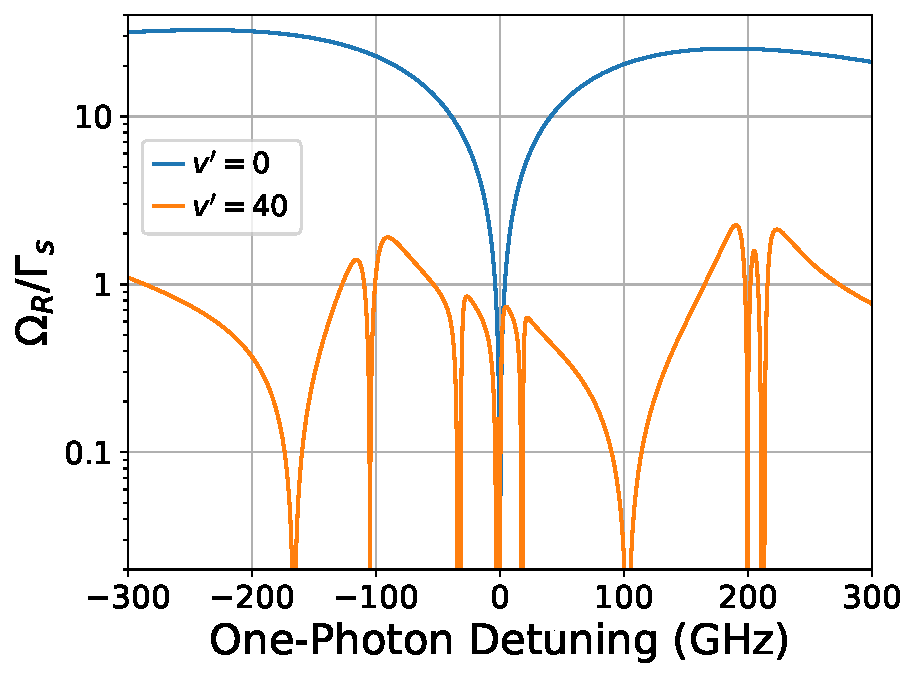
\includegraphics[width=6.4cm]{raman_transfer_theory_ratio_ratio.pdf}};
  \node at (1.225, -2.7) {\scriptsize (\textbf{D})};
\end{tikzpicture}
\end{document}
